\subsection{Fully Connected Neural Networks}
\label{back:linear}

\acrfull{fcnn} are fundamental networks used in many deep learning models. Also called dense-, or linear networks, they are characterized by all neurons between two layers being connected. 
\begin{figure}[!h]
    \centering
    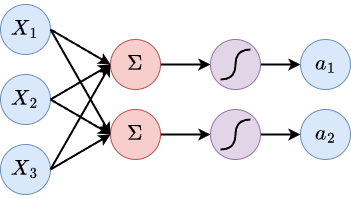
\includegraphics[width=0.5\linewidth]{figures/linearlayer.png}
    \caption{Example of a dense neural network}
    \label{fig:densenn}
\end{figure}


Linear layers perform a linear transformation on the input data, mapping an input vector to an output vector using learnable parameters. The operation can be defined as follows:
\begin{equation}\label{f:wxb}
    y = wx+b
\end{equation}
Here, $x$ is the input vector, $W$ is the weight matrix, $b$ is the bias and $y$ is the output vector.

\begin{figure}[!h]
    \centering
    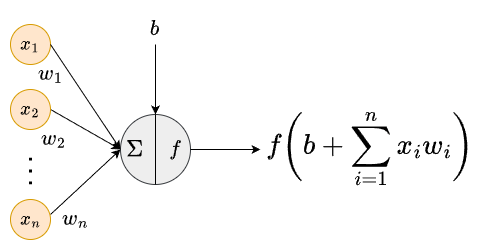
\includegraphics[width=0.7\linewidth]{figures/dl.png}
    \caption{Neurons in a layer with their corresponding weights, a bias $b$ and a non-linear activation function $f$}
    \label{fig:dl}
\end{figure}

Furthermore, an activation function such as $f$ is applied to the output to achieve nonlinearity. By applying $f$ to the output $y$, we now get the equation:
\begin{equation}\label{f:fwxb}
    y = f(wx+b)
\end{equation}

Some of the more popular activation functions include \cite{szandala2021review}: 

\begin{equation}
    Relu(z) = max(0, z)
\end{equation}

Relu (Rectified Linear Unit) has been stated to be the most popular activation functions as late as 2018. Both it's forward and backward pass steps quickly, thus enabling more efficient training compared to other alternatives.

\begin{equation}
    \sigma(z) = \frac{1} {1 + e^{-z}}
\end{equation}

The sigmoid activation is very popular to its very nature of its range being $(0,1)$ compared to other functions where the range is often broader. This makes it good at outputting probibalistic values.

\begin{equation}
    tanh(x) = \frac{e^x - e^{-x}}{e^x + e^{-x}} = \frac{1 - e^{-2x}}{1 + e^{-2x}}
\end{equation}

Similar to sigmoid, the hyperbolic tangent has outputs in a relatively small range $(-1, 1)$
The major bottleneck of all kinds of machine learning tecniques is data. The more diverse and varied a . \\

Linear layers have several advantages, such as computational efficiency, flexibility as well as intrerprebility, where the weight and bias vectors can be interpreted as learned parameters. They also serve as building blocks for other components, such as \acrshort{rnn}s \cite{schmidt2019recurrent}, \acrshort{lstm}s \cite{lstm} or even more novel architectures such as the transformer\cite{vaswani2017attention}. \\ 

However, linear layers have several limitations. Due to their inherent linearity, they are prone to overfitting and struggle to capture complex relationships in data. This can limit their ability to extract more complex features, potentially reducing some of the model's discriminative power. Furthermore, the size of linear layers can become problematic, especially in \acrshort{fcnn}s. Each neuron connection between layers requires storing weights and biases, which increases the overall model size. For a smaller dense network where the layers are of size $[10, 5, 1]$, the total amount of parameters becomes:
$$\begin{aligned}
S &= (10 \times 5 + 5) + (5 \times 1 + 1) \
&= 50 + 5 + 5 + 1 \
&= 61 \text{ parameters}
\end{aligned}$$
Assuming each parameter is stored as a single-precision floating-point number (\texttt{Float32}, 4 bytes), the total memory size is:
$$\begin{aligned}
\text{Memory size} &= 61 \text{ parameters} \times 4 \text{ bytes/parameter} \
&= 244 \text{ bytes}
\end{aligned}$$ While 244 bytes is small, larger dense networks can quickly consume gigabytes of memory. This can create bottlenecks for hardware accelerators like \acrshort{gpu}s, which typically have less VRAM compared to the \acrshort{ram} available to \acrshort{cpu}s.